% Arabic, right-to-left book with LuaLaTeX and babel.
% Fixes found while testing Quarto output:
%  - the sans font (titles) needs Script=Arabic, otherwise letters do not join
%  - code blocks and verbatim output must be English and left to right,
%    otherwise lines and brackets are reversed
%  - selnolig.sty in the project root is an empty stub: the real package breaks Arabic
\babelfont{sf}[Script=Arabic,Renderer=HarfBuzz]{Noto Naskh Arabic}
\addtokomafont{disposition}{\rmfamily}
\usepackage{etoolbox}
\babelprovide[import]{english}
% Numbers set as English runs use the Latin shapes of the same font.
\babelfont[english]{rm}{Amiri}
\AtBeginEnvironment{Shaded}{\bodydir TLT\pardir TLT\textdir TLT}
% Plain blocks (```excel, program output) become fvextra Verbatim so they wrap too.
\AtBeginDocument{\RecustomVerbatimEnvironment{verbatim}{Verbatim}{breaklines,breakanywhere,formatcom={\selectlanguage{english}\pardir TLT\textdir TLT}}}
% Long code lines wrap inside the text width (fvextra), with a small arrow
% at the end of the broken line and the rest indented under it.
\usepackage{fvextra}
\fvset{breaklines=true,breakanywhere=true,breaksymbolleft={\tiny$\hookleftarrow$},breaksymbolindentleft=1.2em}
\AtBeginDocument{\RecustomVerbatimEnvironment{Highlighting}{Verbatim}{commandchars=\\\{\},breaklines,breakanywhere,formatcom={\selectlanguage{english}\pardir TLT\textdir TLT}}}
\setlength{\parskip}{0.45em}
% Cover: the first page of the PDF, built from tex/cover/cover.tex.
\usepackage{pdfpages}
\AtBeginDocument{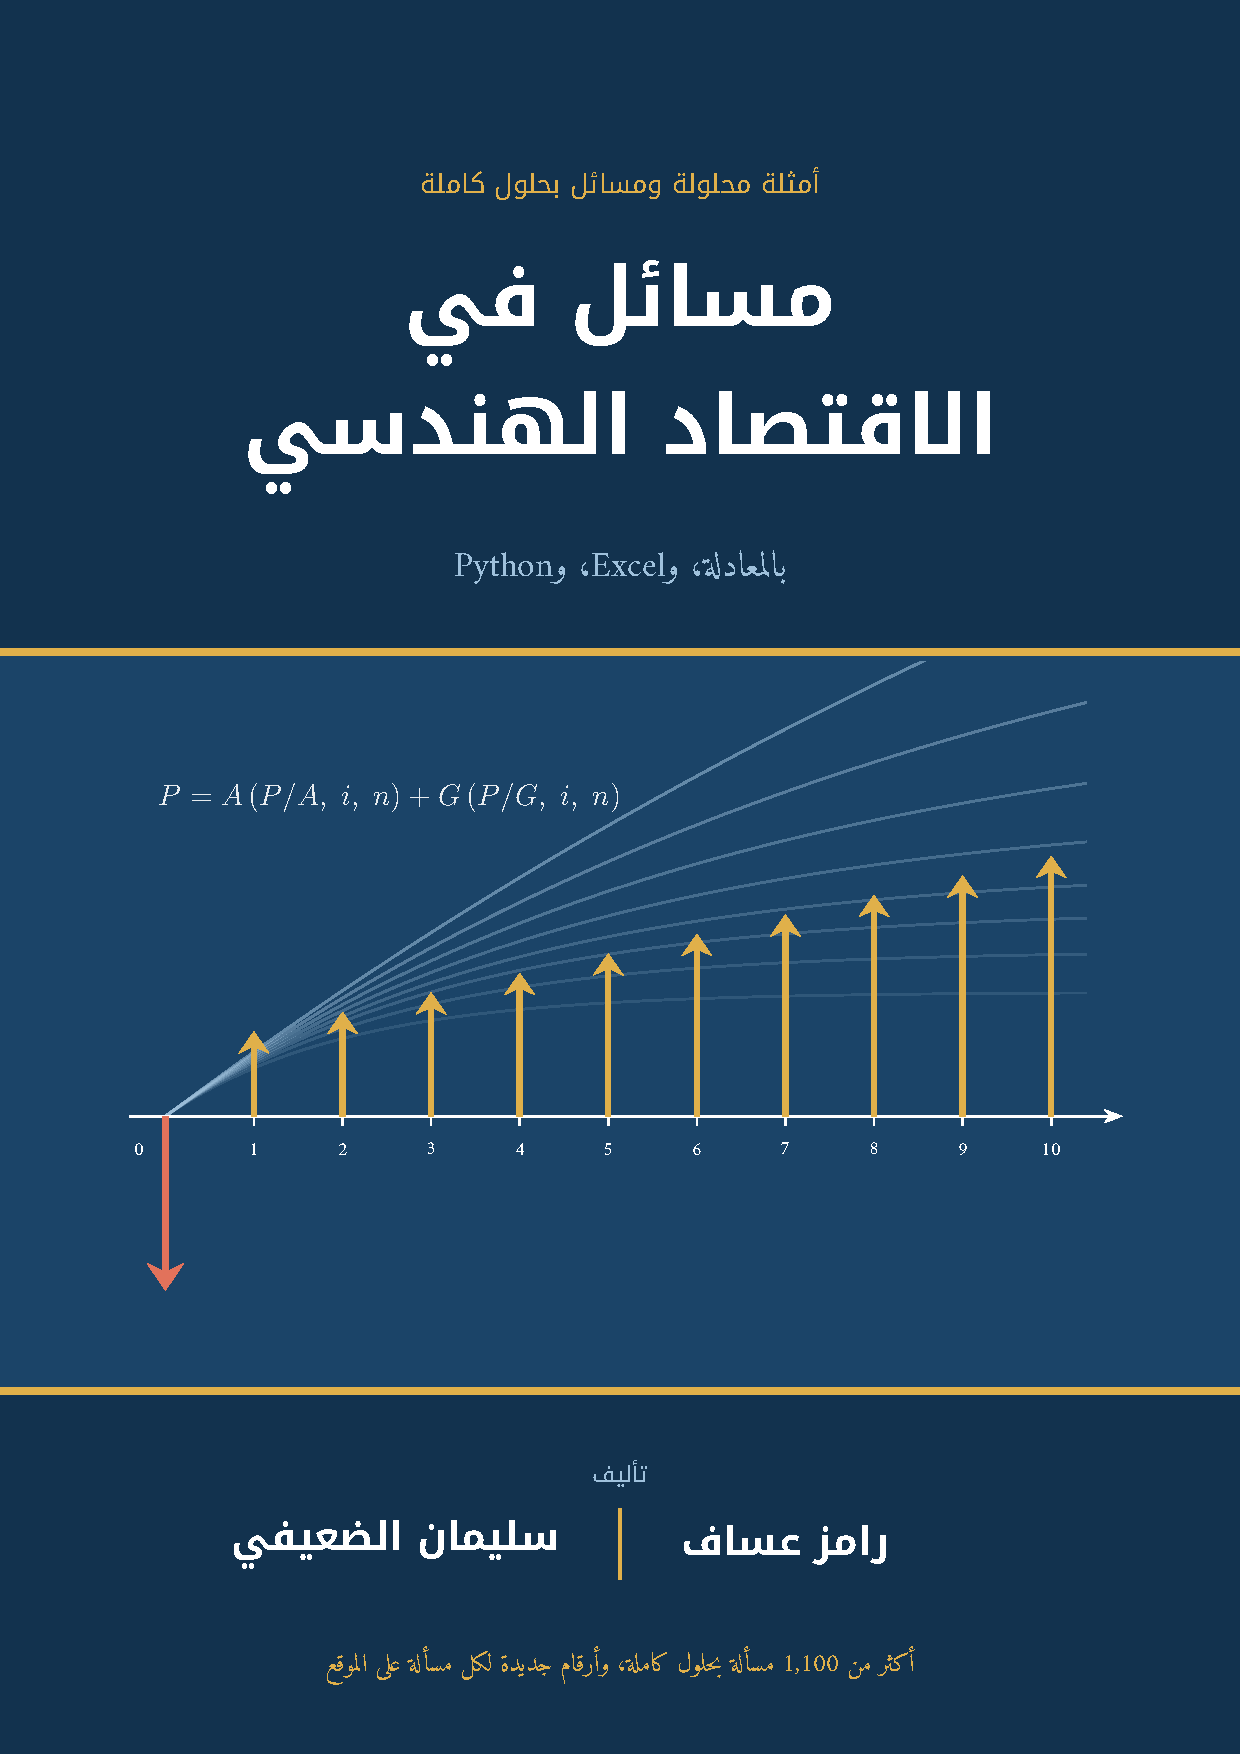
\includepdf[pages=1]{tex/cover/cover.pdf}}

% ---------------------------------------------------------------- colors
% Same palette as the cover. Examples sit in a shaded box with a navy rule on
% the reading side; main equations in a small gold frame (tex/boxes.lua).
\usepackage[most]{tcolorbox}
\definecolor{eeNavy}{HTML}{12324E}
\definecolor{eeExample}{HTML}{EAF1F8}
\definecolor{eeGold}{HTML}{E0B04A}
\definecolor{eeEq}{HTML}{FCF5E3}
\newtcolorbox{exbox}{enhanced, breakable, colback=eeExample, colframe=eeExample,
  boxrule=0pt, arc=2pt, left=8pt, right=8pt, top=4pt, bottom=4pt,
  % the box itself is laid out left to right (tcolorbox draws in that frame), its text right to left
  before={\par\addvspace{9pt}\bodydir TLT\pardir TLT\textdir TLT\noindent}, before upper={\pardir TRT\textdir TRT},
  after={\par\bodydir TRT\pardir TRT\textdir TRT\addvspace{9pt}},
  overlay unbroken and first={\fill[eeNavy] ([xshift=-3pt]frame.north east) rectangle (frame.south east);},
  overlay middle and last={\fill[eeNavy] ([xshift=-3pt]frame.north east) rectangle (frame.south east);}}
% a plain framed box: tcolorbox boxes on a line misplace their frame in right-to-left text
\newcommand{\eqbox}[1]{{\setlength\fboxsep{5pt}\setlength\fboxrule{0.6pt}\fcolorbox{eeGold}{eeEq}{\hspace{4pt}#1\hspace{4pt}}}}
